\documentclass[twocolumn]{article}
\usepackage{fancyhdr}
\usepackage{pgf}
\usepackage{multicol}
\usepackage{amsmath}
\usepackage{enumerate}
\usepackage{listings}
\usepackage[top=2in, bottom=1.5in, left=1in, right=1in]{geometry}
\usepackage{graphicx}
\usepackage{tabularx} 

\lstset{
	tabsize=4,
        basicstyle=\scriptsize,
        %upquote=true,
        aboveskip={1.5\baselineskip},
        columns=fixed,
        showstringspaces=false,
        breaklines=true,
        prebreak = \raisebox{0ex}[0ex][0ex]{\ensuremath{\hookleftarrow}},
	frame=none,
        showtabs=false,
        showspaces=false,
        showstringspaces=false,
        identifierstyle=\ttfamily,
        keywordstyle=\color[rgb]{0,0,1},
        commentstyle=\color[rgb]{0.133,0.545,0.133},
        stringstyle=\color[rgb]{0.627,0.126,0.941},
	language=C++
}

\def\SUBJECT{ECE 486}
\def\TOPIC{Project 2 \\ Branch and Branch Target Prediction}
\def\AUTHOR{Vernon \textsc{Jones} \\ Tyler \textsc{Tricker}}
\def\INSTRUCTOR{Mark \textsc{Faust}}

%*******************Page layout
\pagestyle{fancy}
\lhead{\AUTHOR}
\chead{\SUBJECT: \TOPIC}
\rhead{\thepage}
\fancyfoot{}


\begin{document}
\begin{titlepage}
 \begin{center}
 \newcommand{\HRule}{\rule{\linewidth}{0.5mm}}
% Upper part of the page. The '~' is needed because \\
% only works if a paragraph has started.

\textsc{\LARGE Portland State University}\\[1.5cm]

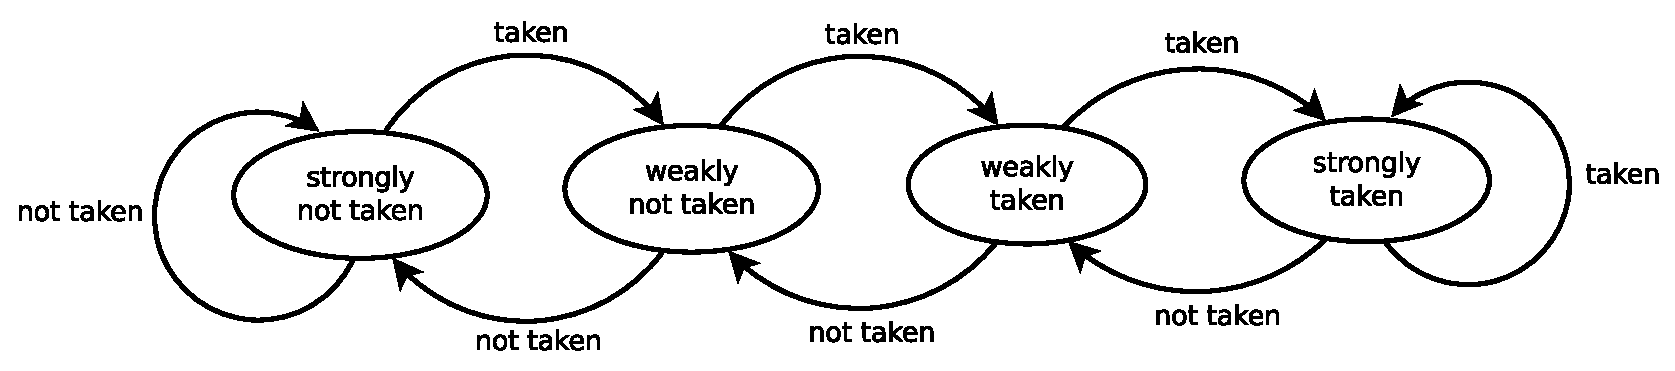
\includegraphics[width=0.5\textwidth]{./logo}~\\[1cm]

\textsc{\Large \SUBJECT}\\[0.5cm]

% Title
\HRule \\[0.4cm]
{ \huge \bfseries \TOPIC}\\[0.4cm]

\HRule \\[1.5cm]

% Author and supervisor
\begin{minipage}{0.4\textwidth}
\begin{flushleft} \large
\emph{Author:}\\
\AUTHOR
\end{flushleft}
\end{minipage}
\begin{minipage}{0.4\textwidth}
\begin{flushright} \large
\emph{Instructor:} \\
\INSTRUCTOR
\end{flushright}
\end{minipage}

\vfill

% Bottom of the page
{\large \today}

\end{center}

\end{titlepage}

\section{Introduction}

\subsection{Branch Target Prediction}

\subsection{Branch Target Buffer}

\section{Method}

\subsection{Trace Analysis}

\subsection{Memory Constraints}

\section{Design}

\subsection{Alpha Predictor}

\subsection{Relative vs Absolute}

\section{Results}
\lstinputlisting{../src/results.log}

\onecolumn
\section{Appendix Code - predictor.h}
\lstinputlisting[language=C++]{../src/predictor.h}
\section{Appendix Code - predictor.cc}
\lstinputlisting[language=C++]{../src/predictor.cc}
\end{document}
